\documentclass[10pt]{hedlab}
\usepackage[utf8]{inputenc}
\usepackage[russian]{babel}
\usepackage[derivative,root,shortcuts]{hedmaths}
\usepackage{graphicx}
\graphicspath{{images/c/}}

\renewcommand\topfraction   {2}
\renewcommand\bottomfraction{2}
\renewcommand\textfraction  {0}

\newcommand{\fiat}{скандия~}
\newcommand{\seat}{молибдена~}

\usepackage{ucs}
\usepackage{listings}
\lstset{
  extendedchars=\true,
  inputencoding=utf8,
  basicstyle=\footnotesize,
  keepspaces=true,
  breaklines=true,
}
\usepackage[usenames,dvipsnames]{color}
\usepackage[colorlinks,linkcolor=black,citecolor=black,urlcolor=Blue]{hyperref}
\renewcommand{\lstlistingname}{Листинг}

\newcommand{\eq}  [1]{\eqref{eq:#1}}
\newcommand{\fig} [1]{\ref{fig:#1}}
\newcommand{\tab} [1]{\ref{tab:#1}}
\newcommand{\sect}[1]{\ref{sec:#1}}

\student{Чечеткин И. А.}
\date{10.04.2014}
\labname{Сечение упругого рассеяния в борновском приближении}
\labnum{3}

\begin{document}
  \makeheader
  
  \section{Аналитические функции экранирования}

  Большинство из предложенных приблизительных аналитических
  функций экранирования основаны на статистической модели
  атома Томаса--Ферми (TФ); есть только несколько исключений,
  основанных на самосогласованных вычислениях Хартри--Фока (ХФ)
  или Хартри--Фока--Слейтера (ХФС). Удобны для дальнейшего
  применения функции экранирования в форме Мольер и Сальвата.
  
  \subsection{Приближение Мольер}

  Уравнение Томаса--Ферми
  \begin{equation}
    \cfrac{d^2\Phi}{dx^2} = \cfrac{\Phi^{3/2}}{x^{1/2}}
    \label{eq:Thomas}
  \end{equation}
  не имеет аналитического  решения, но хорошо аппроксимируется
  формулой Мольер
  \begin{equation}
    \Phi(r)=\sum_{i=1}^3B_i\exp\bigl(-\beta_ir/b\big),
    \label{eq:Moliere}
  \end{equation}
  где
  \[
    B_1 = 0,\!1, \quad B_2 = 0,\!55, \quad B_3 = 0,\!35, \qquad
      \beta_1 = 6,\!0, \quad \beta_2 = 1,\!2, \quad \beta_3 = 0,\!3.
  \]
 
  Функция~\eq{Thomas} отличается от точного решения
  уравнения~\eq{Moliere} меньше чем на 0,\!002 в диапазоне
  \( 0 < x < 6 \).

  \subsection{Приближение Сальвата}

  Использование уравнения~\eq{Thomas} неоправдано, так как оно является
  приближённым. Правильнее было бы использовать уравнение Дирака.
  После решения уравнения Дирака в приближении Хартри--Фока--Слейтера
  (то есть в приближении самосогласованного поля) можно найти
  потенциал и функцию экранирования. Приближение Сальвата
  предполагает использование функции экранирования вида:
  \begin{equation}
    \Phi(r) = \sum_{i = 1}^3 A_i\exp\bigl(-a_ir\big);
    \label{eq:Salvat} 
  \end{equation}
  при этом параметры функции экранирования \( A_i \), \( a_i \) для каждого
  атома индивидуальны. 

  Параметры функции экранирования~\eq{Salvat} находились из
  требования совпадения значений радиальных моментов \( R_n \),
  полученных из нее, с вычисленными методом ДХФС, для
  \( n = -1, 0, 1, 2, 3, 4 \). Это приводит к следующим соотношениям
  \begin{gather}
    A_1 a_1 + A_2 a_2 + A_3 a_3 = R_{-1}, \nonumber \\
    A_1 + A_2 + A_3 = 1, \label{eq:Salvat15} \\
    \frac{A_1}{a_1^n} + \frac{A_2}{a_2^n} + \frac{A_3}{a_3^n} =
      R_n \quad (n = 1,2,3,4). \nonumber
  \end{gather}
  Здесь
  \[
    R_n \equiv \frac{1}{(n + 1)!Z}\int r^n \rho(r)\,d^3r
  \]
  и, в соответствии с уравнением Пуассона,
  \begin{equation}
    \rho(r) = \frac{Z}{4\pi r} \der{\Phi(r)}{r} = \frac{Z}{4\pi r}
      \sum\limits_{i = 1}^3 A_i a_i^2 \exp\bigl(-a_ir\big).
    \label{eq:Poisson} 
  \end{equation}

  Легко видеть, что
  \begin{align*}
    & R_{-1} = \Phi'(0), \\
    & R_0 = \Phi (0), \\
    & R_n = \frac{1}{(n - 1)!} \int\lni r^{n - 1} \Phi(r)\,dr \quad (n \geq 1).
  \end{align*}

  Использование радиальных моментов для определения коэффициентов
  делает сечения рассеяния Борна практически совпадающими с
  вычислеными с помощью экранирующей функции ДХФС. 

  \section{Сечение упругого рассеяния в борновском приближении}

  В борновском приближении для быстрой частицы дифференциальное
  сечение определяется по формуле:
  \begin{equation}
    \der{\sigma}{\Omega} = \frac{4Z^2}{q^4}
      \left[ 1 - \frac{F(q)}{Z} \right]^2,
    \label{eq:diff} 
  \end{equation}
  где \( q \)~-- переданный импульс в столкновении и 
  \[
    F(q) = \int\lni \frac{\sin(qr)}{qr} \rho(r) 4\pi r^2\,dr
  \]
  -- атомный форм-фактор. Для плотности, связанной аналитическими
  экранирующими функциями в форме Мольер и Сальвата, форм-фактор
  принимает простое выражение
  \begin{equation}
    \frac{F(q)}{Z} = \sum_{i=1}^3 \frac{A_ia_i^2}{a_i^2 + q^2}.
    \label{eq:factor} 
  \end{equation}

  Полное сечение рассеяния найдём после интегрирования 
  \begin{equation}
    \sigma = \int\limits_0^{2\pi} d\phi \int\limits_0^\pi \frac{4Z^2}{q^4}
      \left( 1 - \frac{F(q)}{Z} \right)^2 \sin\theta\,d\theta.
  \end{equation}
 
  При упругом столкновении энергия частицы \( E \) не меняется. Это
  значит, что импульс по модулю \\ \( p = \sqrt{2E/m} \) (в атомной системе
  \( p = k = \sqrt{2E} \)) тоже не меняется. В результате
  \( q = 2 k \sin \theta / 2\), где \( \theta \)~-- угол между начальным и
  конечным направлениями импульса. Выполняем замену в интеграле:
  \[
    \frac{q^2}{2k^2} = 1-\cos \theta
  \]

  Получаем полное сечение в виде:
  \begin{equation}
    \sigma = \pi \frac{4Z^2}{E} \int\limits_0^{2k} \frac{1}{q^3}
      \left( 1 - \frac{F(q)}{Z} \right)^2\,dq.
    \label{eq:full}
  \end{equation}

  Подставим в последнюю формулу приближённое выражение \( F(q) \)
  и заменим единицу суммой коэффициентов \( A_i \), получим
  \[
    \sigma = \pi \frac{4Z^2}{E} \int\limits_0^{2k} \frac{1}{q^3}
      \left[ \sum_{i = 1}^3 \left( A_i - \frac{A_ia_i^2}{a_i^2 + q^2} \right)
      \right]^2\,dq.
  \]

  Получаем
  \begin{equation}
    \sigma = \pi \frac{4Z^2}{E} \int\limits_0^{2k}
      \left[ \sum_{i = 1}^3 \frac{A_i}{a_i^2 + q^2}  \right]^2 q\,dq
    \label{eq:sect}
  \end{equation}

  Это выражение имеет то преимущество перед~\eq{full}, что
  не обладает особенностью в 0. Его удобно интегрировать
  численно.
  
  Для представления результатов был написан код на Python.
  Он приведён в разделе~\sect{code}. В его основу легли
  таблицы из работы Сальвата и
  соотношения~\eq{Moliere}--\eq{full}. Результаты численного
  моделирования для атомов \seat и \fiat приведены на
  рисунках~\fig{screening}--\fig{sect}.

  \begin{figure}[h!]
    \centering
    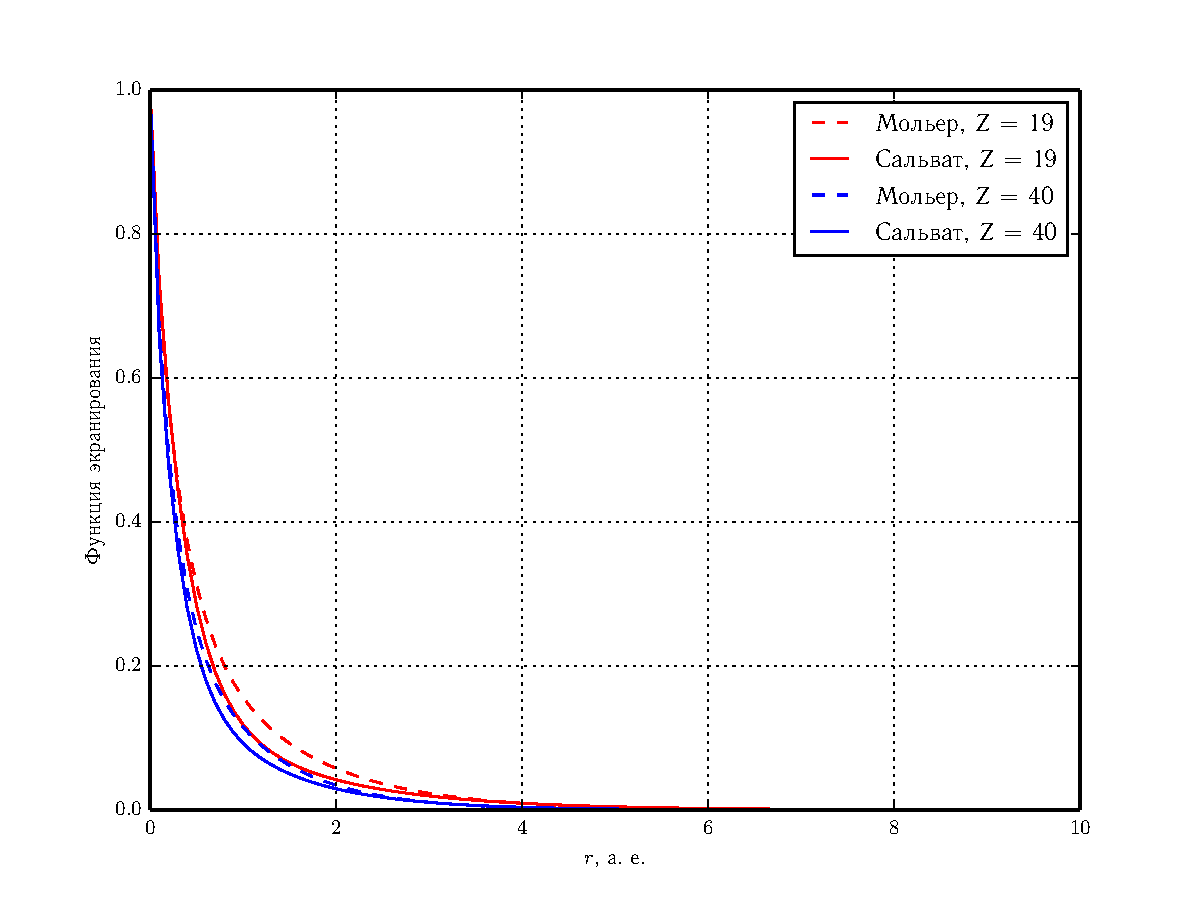
\includegraphics[width=.7\textwidth]{screening}
    \caption{Экранирующие функции для атомов \fiat и
      \seat в приближениях Мольер и Сальвата}
    \label{fig:screening}
    \end{figure}
  
  \begin{figure}[h!]
    \centering
    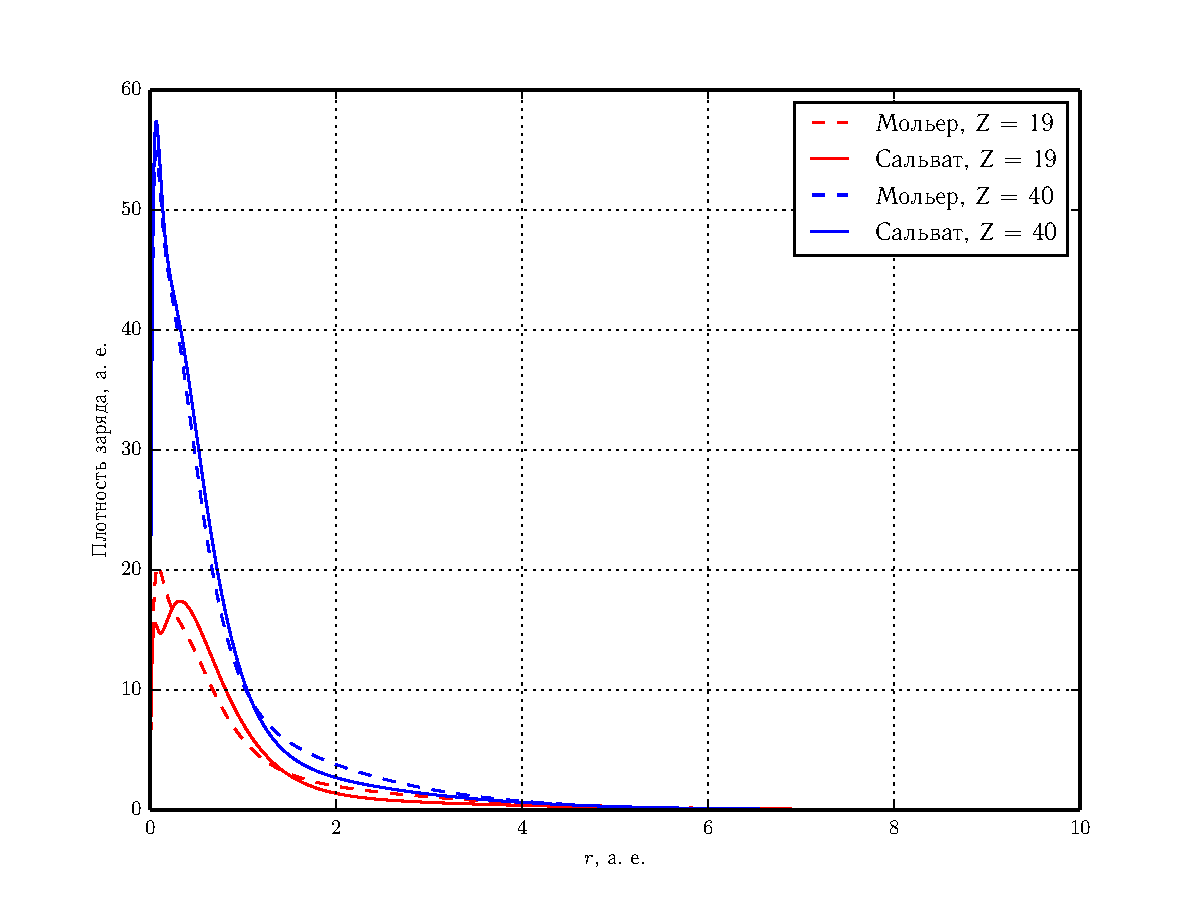
\includegraphics[width=.7\textwidth]{density}
    \caption{Плотность зарядов (электронов) для атомов
      \fiat и \seat}
    \label{fig:density}
  \end{figure}

  \begin{figure}[h!]
    \centering
    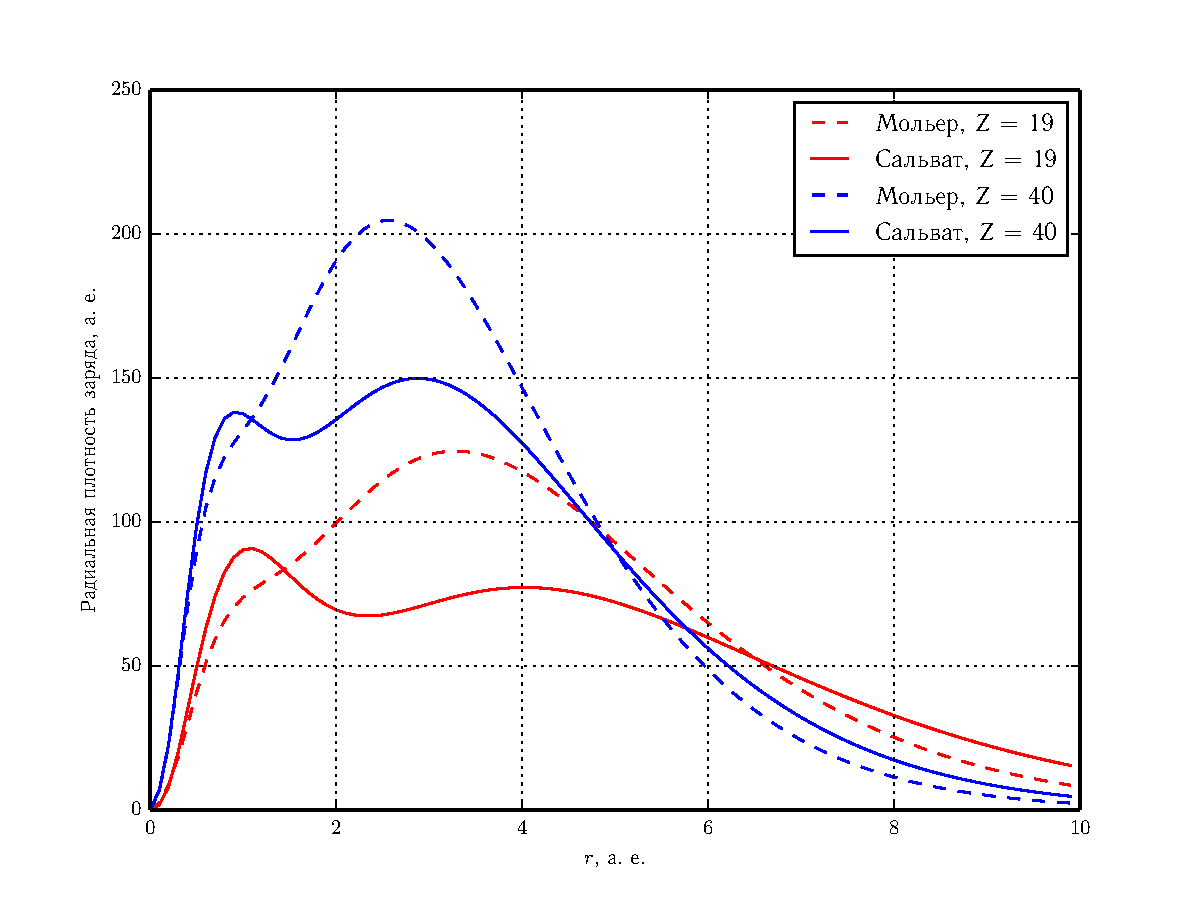
\includegraphics[width=.7\textwidth]{radial_density}
    \caption{Радиальная плотность зарядов (электронов)
      для атомов \fiat и \seat}
    \label{fig:radial}
  \end{figure}
  
  \begin{figure}[h!]
    \centering
    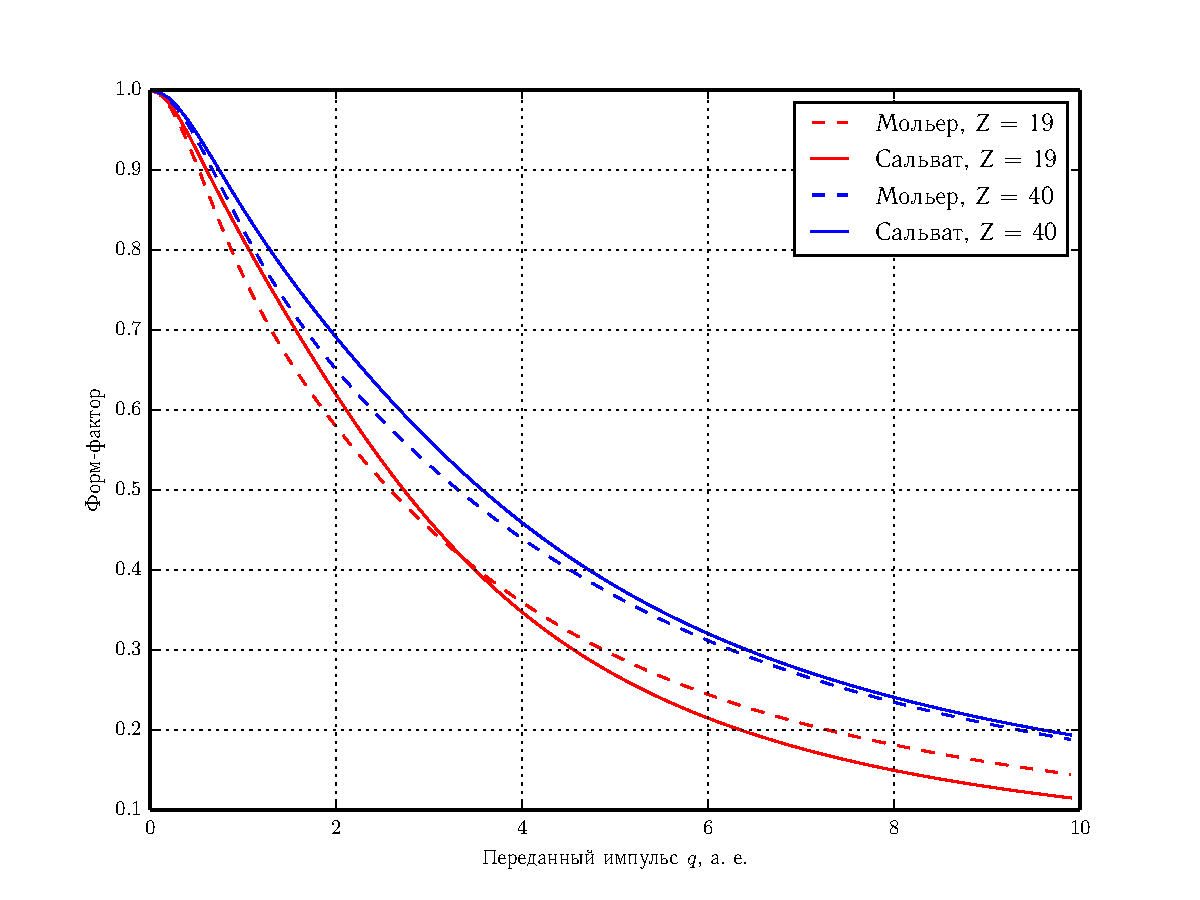
\includegraphics[width=.7\textwidth]{form-factor}
    \caption{Форм-фактор для атомов \fiat и \seat}
    \label{fig:factor}
  \end{figure}
    
  \begin{figure}[h!]
    \centering
    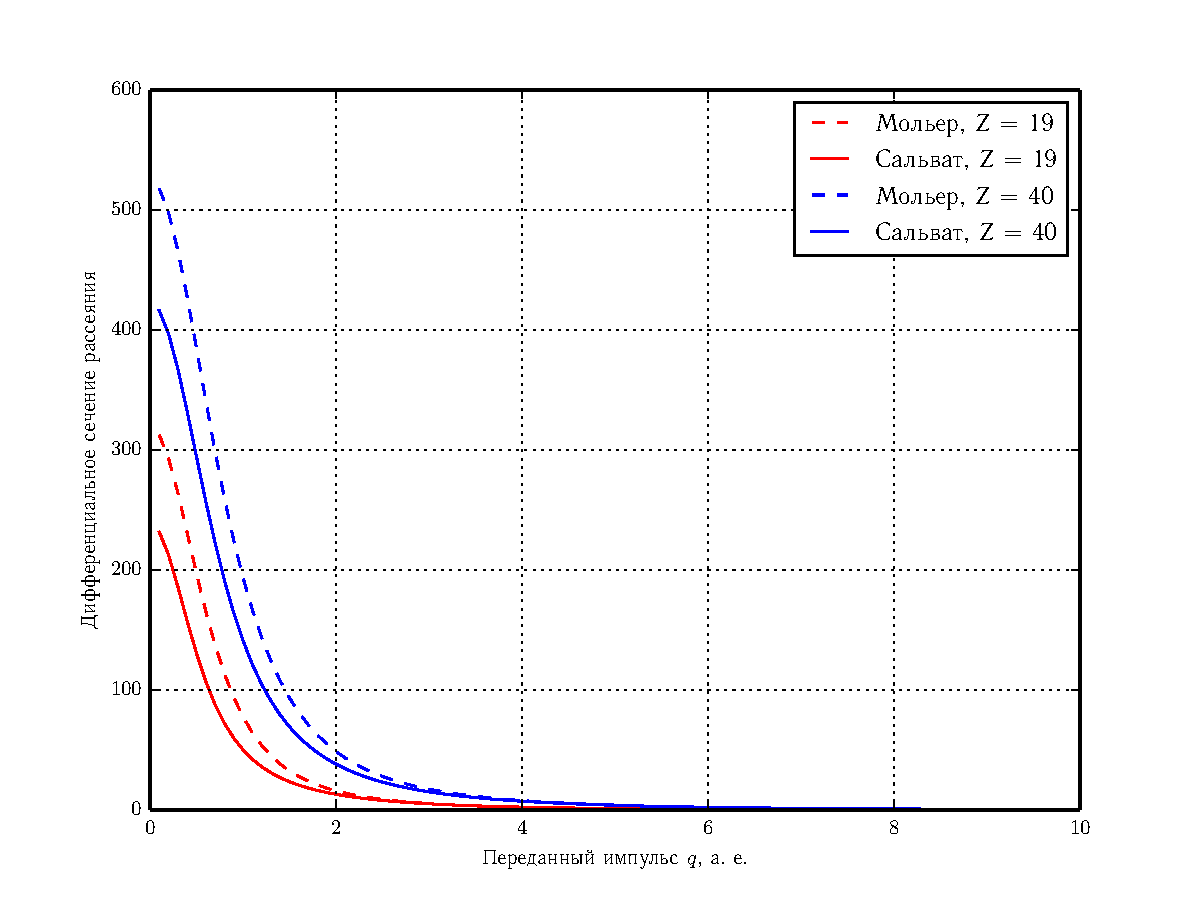
\includegraphics[width=.7\textwidth]{diffsect}
    \caption{Дифференциальное эффективное сечение упругого
      рассеяния электронов в борновском приближении для атомов
      \fiat и \seat}
    \label{fig:diff}
  \end{figure}
  
  \begin{figure}[h!]
    \centering
    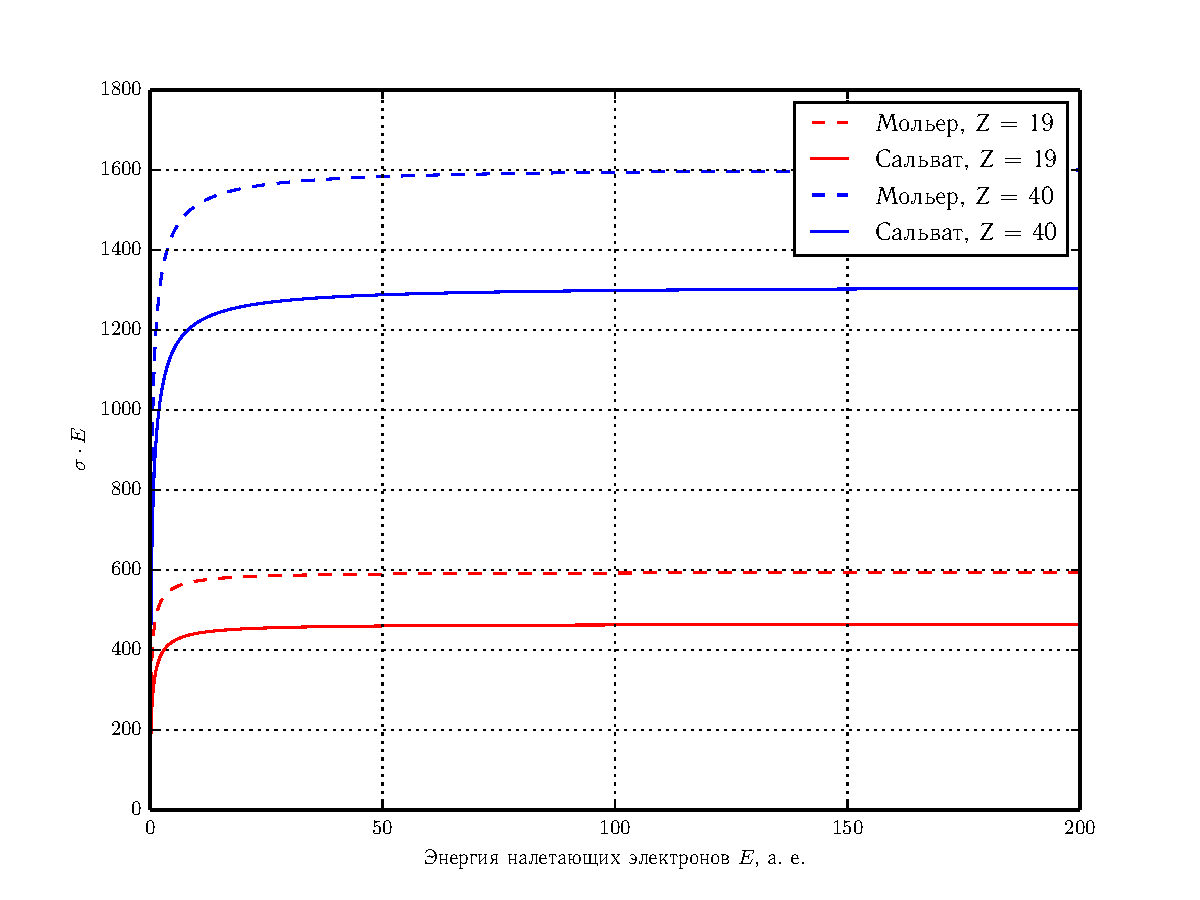
\includegraphics[width=.7\textwidth]{sect}
    \caption{Полное сечение упругого рассеяния электронов в
      борновском приближении для атомов \fiat и \seat в
      приближениях Мольер и Сальвата}
    \label{fig:sect}
  \end{figure}

  \clearpage
  \section{Листинг программы}
  \label{sec:code}  
  \lstinputlisting[language=python]{code/lab3.py}
  
\end{document}
